%\chapter{Design}
%\label{chap:design}
%
%
%In this chapter we introduce a first approach of a visual formalism and later state the final desing of the visual language. Furthermore the idea of automated constraint generation is presented in section~\ref{sec:automatedconstraintgeneration}. The assembly of all the previous features in one tool is described in section~\ref{sec:coalescence}. However, the tool's functionality shall also be available in Robostudio in order to provide safety mechanisms for the healthcare service robots. Section~\ref{sec:integrationintorobostudio} gives a main idea how an integration into Robostudio ought to be. 
%
%%The challenge now is to find a similar intuitive and nonmathematical way of representing reasonable safety constraints for the healthbot domain and to figure out how to translate it to corresponding textual expressions. The new concept will be integrated into Robostudio, a design tool for statemachines, in order to enable the user to create safety constraints visually. A common LTL model checker will be added to it as well which fulfils the verification of the translated constraints on the designed statemachine. In case of verification failures the concerning constraints and a visual counter example can be presented.




\chapter{Visual formalisms for safety constraints}
\label{chap:visualformalismsforsafetyconstraints}

This chapter introduces two different approaches of visual formalisms and later states the final desing of the visual language.
One main difficulty in finding a proper visual formalism is to glean the right level between abstraction and expressiveness since this two characteristics appear to be mutually exclusive in some points. A first approach, so called template constraints,
% and its pros and cons 
are described in section~\ref{sec:templateconstraintformalism}. Subsequently a different design - the operator constraint formalism - is presented in section~\ref{sec:operatorconstraintformalism}.
Section~\ref{sec:comparison} gives a comparison of the two formalisms presented before and states which one is used for the prototype.




\section{Template constraint formalism}
\label{sec:templateconstraintformalism}

%It is not a trivial issue to find a
What visual presentation of constraints would suit a healthbot application developer and what are the main types of safety constraints he could want to check?
% TODO: wir haben gedacht, dass es einfach zu benutzen ist
Led by this question, a visual language based on templates has been developed. These templates make different propositions about states and their relations. The user can choose from several graphical constraint types and customize them by parameterising state variables. So far there are two different kinds of template constraints:

\begin{enumerate}
	\item Whenever state (x) is active, state (y) must be visited before state (z) can be reached.
	
	The idea behind this constraint is that propositions about temporal dependencies can be made. Under certain circumstances a visit of a particular state is restricted as long as a specific precondition is fulfilled. An example constraint for this template is: Whenever a person is eating (x), he must brush his teeth (y) before he can go to bed (z). Thus, going to bed without brushing teeth after meal should never happen.
	\item Each visit of state (x) will eventually result in a visit of either state (y) or state (z) [or state (w) [...]]. All of them are actually reachable.
	
	This constraint type enforces at least one particular event to happen after a specific precondition.
	An example of such a constraint would be: Every time a person enters a supermarket (x) he will eventually decide to buy 
	%a product or not to buy it.
	something (y) or to leave the shop with empty hands (z). He finally has to make a decision, but he can not avoid both possibilities.
	%Nitpicking readers might note 
	Of course the person could also steal something without buying it, and thus not buy anything but leave the shop with full hands. In fact, exactly in this case the constraint would signal an undesirable ``program'' behaviour with its invalidity.
\end{enumerate}

Figure~\ref{fig:templateconstraints} gives a visual suggestion how the two constraint types could look like. Each state of a constraint is symbolized by the robot surface to make the user think he's directly working with the robot. Furthermore the state labels could be replaced by the real screen displays of the regarding states. All parameters of the template constraints shall be directly customizable by the robot surface symbols. Figure~\ref{fig:templateconstraint_dropdown} demonstrates how states could be choosen as parameters.
 
\begin{figure}[htbp]
  \centering
  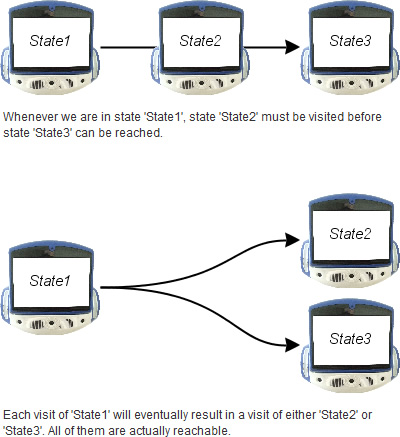
\includegraphics[scale=0.7]{templateconstraints}
  \caption{The two template constraint types, parameterized with particular states.}
  \label{fig:templateconstraints}
\end{figure}

\begin{figure}[htbp]
  \centering
  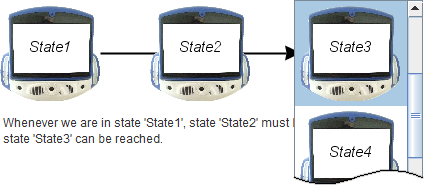
\includegraphics[scale=0.7]{templateconstraint_dropdown}
  \caption{Possible way of specifying template parameter.}
  \label{fig:templateconstraint_dropdown}
\end{figure}

All template constraints are additionally equipped with textual expressions in order to explain their semantics. It is a template sentence with placeholders for the states available for parameterisation. Whenever there is a change to the constraint, te text is being updated automatically regarding to the parameter states. These additional expressions are also shown in figure~\ref{fig:templateconstraints}.

Each template constraint describes a certain behaviour which might be later used for checks. Thus, specific formulas have to be provided which represent the semantics of the constraints. They have to be in a format so that they can be processed by a model checker. For the first kind of template operator, a linear temporal logic fomula (LTL, see~section~\ref{sec:modelcheckingandltl}) expresses its semantics (with $x$ as ``x is current state'' and similarly for $y$ and $z$):

\begin{equation} \label{eq:template_one}
  \models \Box (x \rightarrow ([(\neg z) \mathcal{U} y] \vee \Box \neg z))
\end{equation}

``Globally is true: Whenever x is the current state, either z is not visited until y or z is never visited''. Compared to the example above it means: Whenever a person eats something (x), he can not go to bed (z) until he brushes his teeth (y). Otherwise, if he never goes to bed, he does not necessarily need to brush his teeth.

The semantics of the second operator template is more complex since it has a secondary condition that all y, z, ... states are actually reachable after a visit of x. Possibilities can not be expressed by LTL, thus, it needs to use computation tree logic (CTL) for describing this auxiliary condition in a second formula. A short explanation about CTL is already given in section~\ref{sec:delbimbo}, but the two new constructs used for this formula are described below.
The main formula for the second template is still using LTL:
\begin{equation} \label{eq:template_two_one}
  \models \Box (x \rightarrow \Diamond (y \vee z (\vee ...)))
\end{equation}
``Globally is true: Whenever x is the current state, in a future step either y or z (or ...) will be visited''. In context of the example mentioned above it means: Every time a person enters a supermarket (x) he will eventually buy something (y) or buy nothing (z). The fact that both states are really potentially reachable is expressed by the following CTL formula. \emph{AG} replaces the $\Box$ sign and stands for ``on all paths is globally true...'', \emph{EF} is related to $\Diamond$ and expresses ``a path exists where is true in future...''.
\begin{equation} \label{eq:template_two_two}
  \models AG (x \rightarrow ((EF y) \wedge (EF z) (\wedge ...)))
\end{equation}
``It is globally true on all pahts: Whenever x is the current state, there is at least one path leading to y and at least one path leading to z''.








\section{Operator constraint formalism}
\label{sec:operatorconstraintformalism}

The operator constraint formalism is a new approach with a special focus on expressiveness and uniqueness of the visual language.
%For this the abstraction level is adapted in order to 
It is designed as a visual formalism for linear temporal logic having a visual operator for each LTL operator. Since the visual constraints are directly mapped to LTL expressions, the visual language is equal to LTL in expressiveness. If it is considered as easy to use, non-experts can use it as well as experts who already know LTL.


\subsection{Requirements}

To provide the required functionality, the fundamental logical operators are required, as shown in (a) through (e) below.

\begin{description}
	\item[(a)] \emph{AND} operator: $\varphi \wedge \psi$.
	\item[(b)] \emph{OR} Operator: $\varphi \vee \psi$.
	\item[(c)] \emph{IF} operator: $\varphi \rightarrow \psi$.\\Instead of an \emph{IMPLIES} operator an \emph{IF} operator is provided. Its meaning seems to be more intuitive for non-experts since it is a common construct in almost every programming language.
	\item[(d)] \emph{NOT} operator: $\neg \varphi$.
	\item[(e)] Proposition: $\rho$.\\Until now there is only the \emph{state proposition} type, which gives evidence about the currently active state. Other types such as numeric or string equations may be added but are less important for the healthcare subject.
\end{description}
	
In addition to these five logical operators the visual language should be furthermore capable of expressing constraints about future steps, both ``any future state'' (h) and ``the next state'' (g), that ``events should always happen'' (f), and that ``a property must be true until some future event'' (i).
	
\begin{description}
	\item[(f)] \emph{ALWAYS} operator: $\Box \varphi$.\\$\varphi$ must be true now and in all following states.
	\item[(g)] \emph{NEXT} operator: $\medcircle \varphi$.\\$\varphi$ has to be true in the next state.
	\item[(h)] \emph{FUTURE} operator: $\Diamond \varphi$.\\At least one time - now or in a later state - $\varphi$ must be true.
	\item[(i)] \emph{UNTIL} operator: $[\varphi \mathcal{U} \psi]$.\\Now and in all following states $\varphi$ must be true at least until there is a state with $\psi$ being true. In addition eventually there has to be a future state with $\psi$ being true.
\end{description}

All the operators mentioned above shall be suitable for constraint editing in a way that the visual language is very easy to use, especially for non-experts. This implies simple editing as well as easy readability of constraints. Furthermore it should provide an intuitive application which is ideally learnable within little time.





\subsection{Design decisions}

Like the formula representation introduced by Del Bimbo et al.~\cite{520786}, a constraint consists of nested operators and propositions in a hierarchy. However, the new visual formalism surrenders the three dimensional idea and focuses on two dimensional blocks and their compositions instead, which is used by HomeTL~\cite{4341725} as well. Each operator of the visual language is represented by such a block.

The visual language has support for eight unary or binary operator types and one proposition which have their specific semantics. In order to support the reading of constraints, different significant visual appearances of the operator types shall enable easy classification and a faster subconscious identification~\cite{moody-physics-of-notations}. In this case, different colors are used for each operator type.
% aiming for faster perceptibility and understandability. 
A suggestion for the operators' graphical representation is shown in figure~\ref{fig:operators}.

\begin{figure}[htbp]
  \centering
  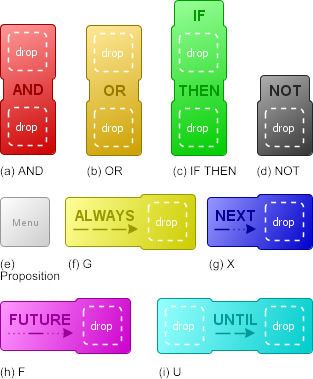
\includegraphics[scale=0.65]{table}
  \caption{Visual representation of all supported operators.}
  \label{fig:operators}
\end{figure}

A second effort for making the perceptibility of the visual language as intuitive as possible is done with the orientation of constraints. 
Operators which consist of nested operators have particular meanings for the two dimensions: The ``logical'' vertical read direction and the horizontal direction for variation in time. Thus, logical operators are arranged in a vertical row wereas time relevant operators are aligned horizontally.
Figure~\ref{fig:directions} demonstrates an example constraint composed along the logical and time axes.
\begin{figure}[htbp]
  \centering
  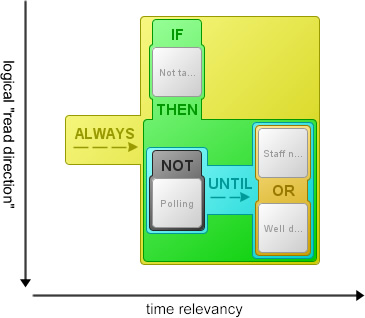
\includegraphics[scale=0.65]{directions}
  \caption{Easy understanding of visual constraints due to intuitive read directions.}
  \label{fig:directions}
\end{figure}
It is read from left to right and top to bottom:
``ALWAYS is true: IF state \emph{'Not taken yet'} is active THEN state \emph{'Polling'} can NOT be visited UNTIL state \emph{'Staff notified'} OR state \emph{'Well done!'} is reached.''

The two dimensions form a special requirement also for the layouting of nested operators. Each operator adapts its size so that it surrounds all recursively nested operators. But also the positioning of nested operators within teir parents have to be taken into account.
Whereas the operator's centered positioning and resizing along the logical direction only depends on the sizes of all sub operators, the arrangement within the time axis turns out to be more complex. Here, sub operators can not just be aligned centered as it is the case vertically. To face the determination of horizontal positioning, every operator gets time reference lines which specify its positioning within its parent and the positioning of its own children within itself. As depicted in figure~\ref{fig:referencelines}, logical operators - i.e. \emph{IfThenOperator}, \emph{AndOperator}, \emph{OrOperator}, \emph{NotOperator} and \emph{StateOperator} - have one reference line. Time relevant operators - i.e. \emph{NextOperator}, \emph{FutureOperator}, \emph{AlwaysOperator} and \emph{UntilOperator} - have two such reference lines, one for their own positioning within their parents and one for the positioning of their children.

\begin{figure}[htbp]
  \centering
  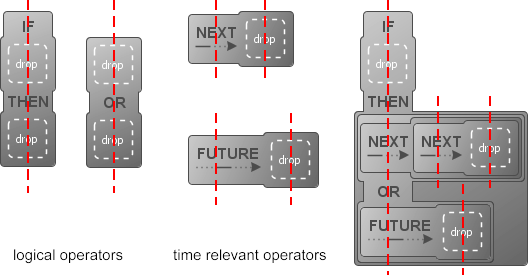
\includegraphics[scale=0.65]{referencelines} 
  \caption{Time reference lines and their adjustments.}
  \label{fig:referencelines}
\end{figure}

As postulated in the requirements for the visual language, constraints shall be easy to read. In fact, there is a possibility to improve the presentation of certain visual constraints. Multiple nested operators of the same kind which have no order priorities such as \emph{OR} or \emph{AND} appear graphically unnecessarily complex. These operators can be visually merged in the manner of unifying their border lines, for example. As a result, all associated operators appear as just one operator with a couple of sub operators (see~figure~\ref{fig:nested_and}).

\begin{figure}[htbp]
  \centering
  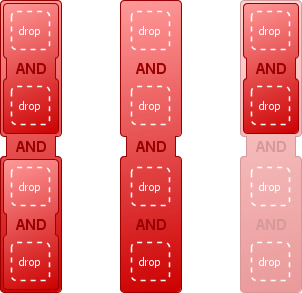
\includegraphics[scale=0.65]{and_simplify}
  \caption{Default nested \emph{AND} operator and visually merged nested \emph{AND} operator.}
  \label{fig:nested_and}
\end{figure}		







\subsection{Guidelines for an editor}

Also an editor for this visual language which holds the functionality for composing operators can contribute to usability and clarity. Some requirements are as follows:

\begin{itemize}	
	\item All editing is performed only by simple drag and drop. Operators and propositions can be moved and dropped onto other operators. A tool bar provides all operator and proposition types to be instantiated and a possibility for deleting existing operators.
	\item In order to simplify the reading of constraints an operator can be hovered over by the mouse pointer. It is intended to be similar to line coloring when reading a digital text.
	\item Every edit to either the constraint or the underlying state machine results in an automatically (re-)validation of the constraint. The result is immediately displayed to the user.
	\item There is no button for constraint creation / editing except operator and proposition providers, which let the developer create new instances. Having no additional buttons reduces complexity and keeps it simple.
\end{itemize}









\section{Comparison}
\label{sec:comparison}

Due to its arrow based design the visual language for template constraints is a good visualisation of time dependencies. Furthermore, it allows expressing possibilities by the use of CTL formulas which is not possible with the operator costraint formalism.
Nevertheless, the template visualisations have some trouble with clearness of their semantics. Even though there are well defined formulas behind each constraint and textual expressions which explain the meanings of constraints, the visual presentation seems to be ambiguous in some settings what leads to the risk of being interpreted differently. For example, in the context of the visual language it is unclear whether the first constraint template allows state (x) to be visited more than once before state (z) is reached. It might also be problematic to interprete whether more than one of the states $y$, $z$, ... can be actually visited after a visit of $x$ in the second constraint. In contrast, the operator constraint formalism is not ambiguous due to to its direct mapping to LTL wich is consistently defined. All visual operator expressions represent exactly the same semantics as their corresponding textual LTL formulas.

%The visual language for template constraints was presented to potential users for evaluation and feedback. Though most of them named it a good concept, soon it turned out that they had problems and disagreements concerning the issues mentioned above. The presented constraints were interpreted differently, the meaning seemed to be unclear and ambiguous. 

However, there is a second problem with the template constraints.
Whereas the safety constraints specific to the example within the healthcare domain mentioned in section~\ref{sec:healthbotapplication} are expressable by this visual language, there are other common constraints which have no matching template and thus can not be described. For example, the check of a state being visited never or at least once is not possible. For every new constraint type a new template has to be created what means an infinite amount of templates is needed in order to achieve full expressiveness.
On the contrary, the visual language for operator constraints is not limited in expressiveness compared to LTL, disregarding that there is only one proposition type available. But this is an extension issue of the prototype rather than a lack in expressiveness.
% Gefundene probleme, die man erw�hnen k�nnte: beim if operator ist das �bergeordnete always nicht intuitiv. der always operator k�nnte umgedreht sein.

Since a visual language has to be developed which suits non-professionals as well as experts, the risk of ambiguity is undesirable. Especially for a tool for safety and consistency it would form a really bad basis. For this reason, the approach of template constraints is discarded and the operator constraint formallism is used for the editor prototype instead.
Owing to the recursive nesting of operator constraints, a visual formula can be recursively translated to a LTL sentence which can be processed by the prototype using any ordinary model checker.